\documentclass[10pt,twoside,english,a4paper]{article}

\usepackage[english]{babel}
\usepackage[IL2]{fontenc}
\usepackage[utf8]{inputenc}
\usepackage{graphicx}
\usepackage{url}
\usepackage{hyperref}
\usepackage{cite}
\usepackage{times}
\usepackage{indentfirst}
\usepackage{multirow}

\pagestyle{headings}

\title{The influence of video games on people and the human psyche\thanks{Semester project in the subject Methods of engineering work, ac. year 2022/23, management: Ing. Igor Stupavsky}}

\author{Erik Roganský\\[2pt]
	{\small Slovak University of Technology in Bratislava}\\
	{\small Faculty of Informatics and Information Technologies}\\
	{\small \texttt{xrogansky@stuba.sk}}
	}

\date{\small December 07, 2022}


\begin{document}

\maketitle

\begin{abstract}
This paper presents a summary of video games and their influences on people and the human psyche. The correlations between a diversity of issues but also benefits and video games are undeniable. Different video game genres have varying effects on how sympathetic individuals are. Some are harmful, some the other way around. Video games can help you socialize in a way, but on the other side, they degrade children's in-person communication skills. Their captivating tendency has great potential in education and skill improvement but can also lead to getting addicted, overweight, sleep deprived, and much more. With fast-advancing times and generations rapidly changing, video games can easily cause even problems with sexuality. It is imperative to be aware of both the benefits and the risks associated with video games to be able to approach playing them safely and, most importantly, healthily.
\end{abstract}



\section{Introduction} \label{introduction}
Over the last few, video games have started to gain popularity, and the increase is far from stopping. In the past, not many people could afford to play video games. Computers were exceedingly expensive, and gaming consoles were no better. As time passed, electronic devices became more affordable for everyone. The age range of video game players is also expanding precipitously (see Table 1). Video games, in general, were designed to entertain teenagers and young adults. These days, it is not uncommon to find a toddler playing with a smartphone, a mature adult sitting in front of television playing games on a console, or even an elder, playing on a computer. As video games are expanding among more and more people, their influence, whether it is positive or negative, is also getting more vast. That is why we should focus more on the issue of video games and their impacts on humans, which will be the main topic of this work.

\begin{table}[h]
\centering
\begin{tabular}{ |p{3cm} r| }
 \hline
 \multicolumn{2}{|c|}{Distribution of video gamers in the} \\
 \multicolumn{2}{|c|}{United States in 2022, by age group} \\
 \hline
 Characteristic & Share of respondents\\
 \hline
 Under 18 years & 24\%\\
 18-34 years & 36\%\\
 35-44 years & 13\%\\
 45-54 years & 12\%\\
 55-64 years & 9\%\\
 65+ years & 6\%\\
 \hline
\end{tabular}
\caption{A table of percentage of video game players age (taken from ~\cite{age2022})}
\end{table}

\section{Influence on empathy and behavior} \label{empathy}
Empathy is one of the most important characteristics to possess, and it literally sets humans apart from other animals. Empathy is one of the most important characteristics to possess, and it literally sets humans apart from other animals. The definition of empathy could be "the capacity to comprehend and partake in the emotional condition or situation of another."~\cite{empathy}.

Since everybody is different, they also behave and are empathic differently. Empathic levels and behavior can be influenced by one's background, location of residence, school, friends, family, and virtually anything from the outside world. Also, it applies to video games. The best examples are violent and prosocial video games.

\subsection{Violent video games} \label{violent}
Games containing a violent undertone are among the most popular genres of video games. Whether they are shooters or there is physical violence included, they all have the same impact on humans. They lead to lower levels of prosocial behavior and a decrease in empathy~\cite{empathy}. In the worst-case scenario, violent video game players may turn antisocial and exhibit sociopath-like behaviors. Violent games do, however, have a good side as well, which will be mentioned later on.

\subsection{Prosocial video games} \label{prosocial}
On the other hand, there are games that can be called prosocial. Their prominent focus is on in-game helping and cooperation. They restrain aggression by attenuating the connection between aggressive cognition and aggressive behavior. Therefore they enhance prosocial behavior in humans~\cite{empathy}. In other words, those who participate in these games act more kindly toward others, adhere to the law more consistently, and are generally seen as decent, well-behaved, and helpful people.

\section{Positive effect on humans} \label{pozitive}
Growing popularity makes video games an excellent tool that can be used in various positive ways. They have the power to improve the quality of life in an abundance of aspects. Some studies, for example, researched how violent games affect people, and the outcome is remarkable. They found out that games containing violence do not lead to aggression but, on the contrary, improve visuospatial skills. Another study discovered that seniors who regularly or at least occasionally play video games witness better well-being and experience less depression than those who do not~\cite{poz-neg-sol}.

\subsection{Socializing via video games} \label{socializing}
As far as society remembers, games played a vital role in socializing. The first game is dated back to ancient times. People played games to meet others and to entertain each other. People created many meaningful bonds through playing games. As time has passed and we have come to a digital era, video games have started to dominate over classical games. In the matter of socializing, MMO (Massively Multiplayer Online) games are one of the best ways to meet people online. They are designed to be social on a massive scale. MMO games are technically a space with hundreds of people that play together, competitively or cooperatively. While meeting people via video games may not be the same as shared experiences, friendships established through playing video games can be similarly meaningful~\cite{poz-neg-sol}. Additionally, people having difficulties establishing normal relationships can also benefit from playing these games because they make it for them to talk through the game than face to face.

\subsection{Education} \label{education}
Video games have a great tendency to capture people's attention and hold it for long periods of time. On the other hand, learning by itself has the exact opposite effect. These two elements are combined in video game-based learning, which makes it a remarkable learning strategy. But it's important to remember that video games should not be the primary method of education and should only be utilized as a learning aid. There are video games with solely educational purposes, despite the fact that creating such is challenging. Counting, writing, spelling, and pronouncing activities for young children and toddlers are a few examples. Then there are games still being considered educational but aren't designed to teach their players something new, but they help players enhance their already existing abilities. For instance, sudoku helps improve logic, crosswords aid with vocabulary expansion, and Millionaire helps with general knowledge improvement, along with a multitude of other games~\cite{learning}.

\subsection{Ability improvement in other video games} \label{improvement}
Even games that are not intended to teach anything can be of benefit. A study shows that almost every video game genre can be beneficial for something. Adventure games are the most common illustration. A compelling plot, action, problem-solving, riddles, puzzles, and many kinds of seeking for things are nearly always included~\cite{learning}. All these things by themselves can improve specific abilities. For instance, the action in adventure games enhances quick reactions (see Figure 1). Strategy games, on the other side, improve one's decision-making skills and thinking abilities. There are a handful of video game genres that can help with improving something, but that is a story for another time. 

\begin{figure}[h]
\centering
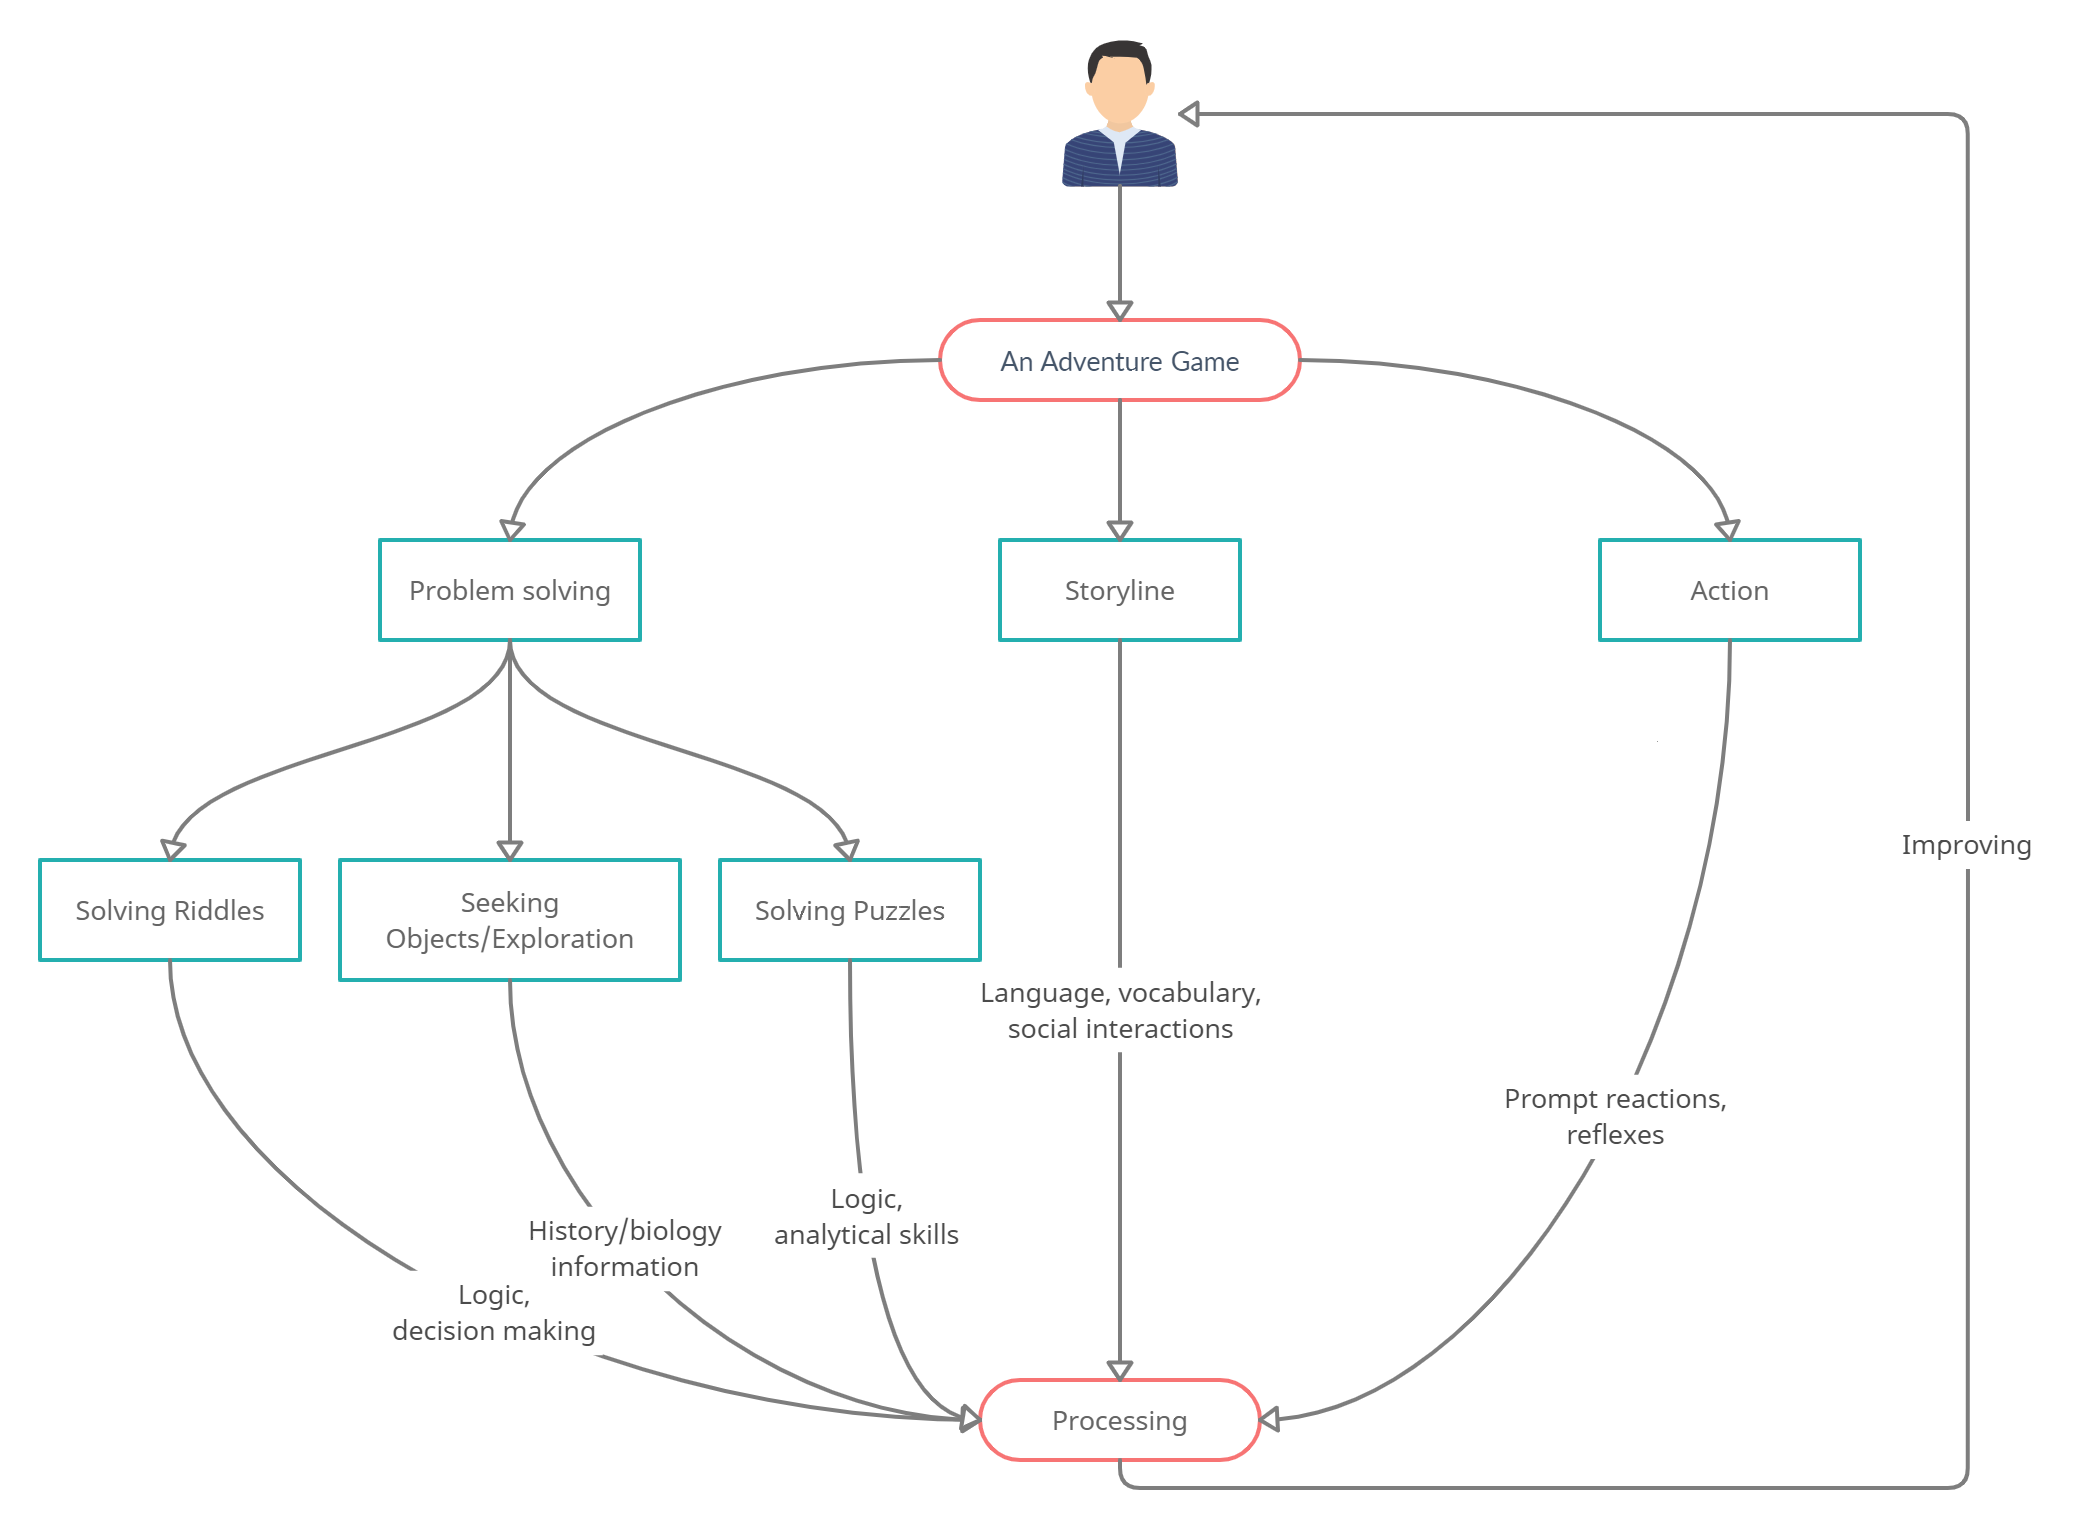
\includegraphics[scale=0.27]{adventure}
\caption{A diagram of how adventure games help improve certain abilities}
\end{figure}

\subsection{Foreign language learning} \label{language learning}
Despite the fact that video games are still not as successful in the classroom as they could be, they may be significantly beneficial for language acquisition. Numerous studies back up the concept of learning foreign languages through video games but ideally in conjunction with conventional learning methods. Video games' ability to engross their players has been found to be an excellent tool for language learning. They contain endless dialogues in oral and written form (see Figure 2). It is easier to understand the words and sentences since players have substantial control over their in-game actions, decisions, and dialogue choices~\cite{language}. Even the possibilities to pause the game, repeat certain moments, or select alternate options are advantageous. Video games give more vocabulary repetition than movies or books do. For instance, in mini-battles, shooting, solving puzzles, or even in the game menu~\cite{language}. As is well known, repetition is one of the most effective methods for language learning.

\begin{figure}[h]
\centering
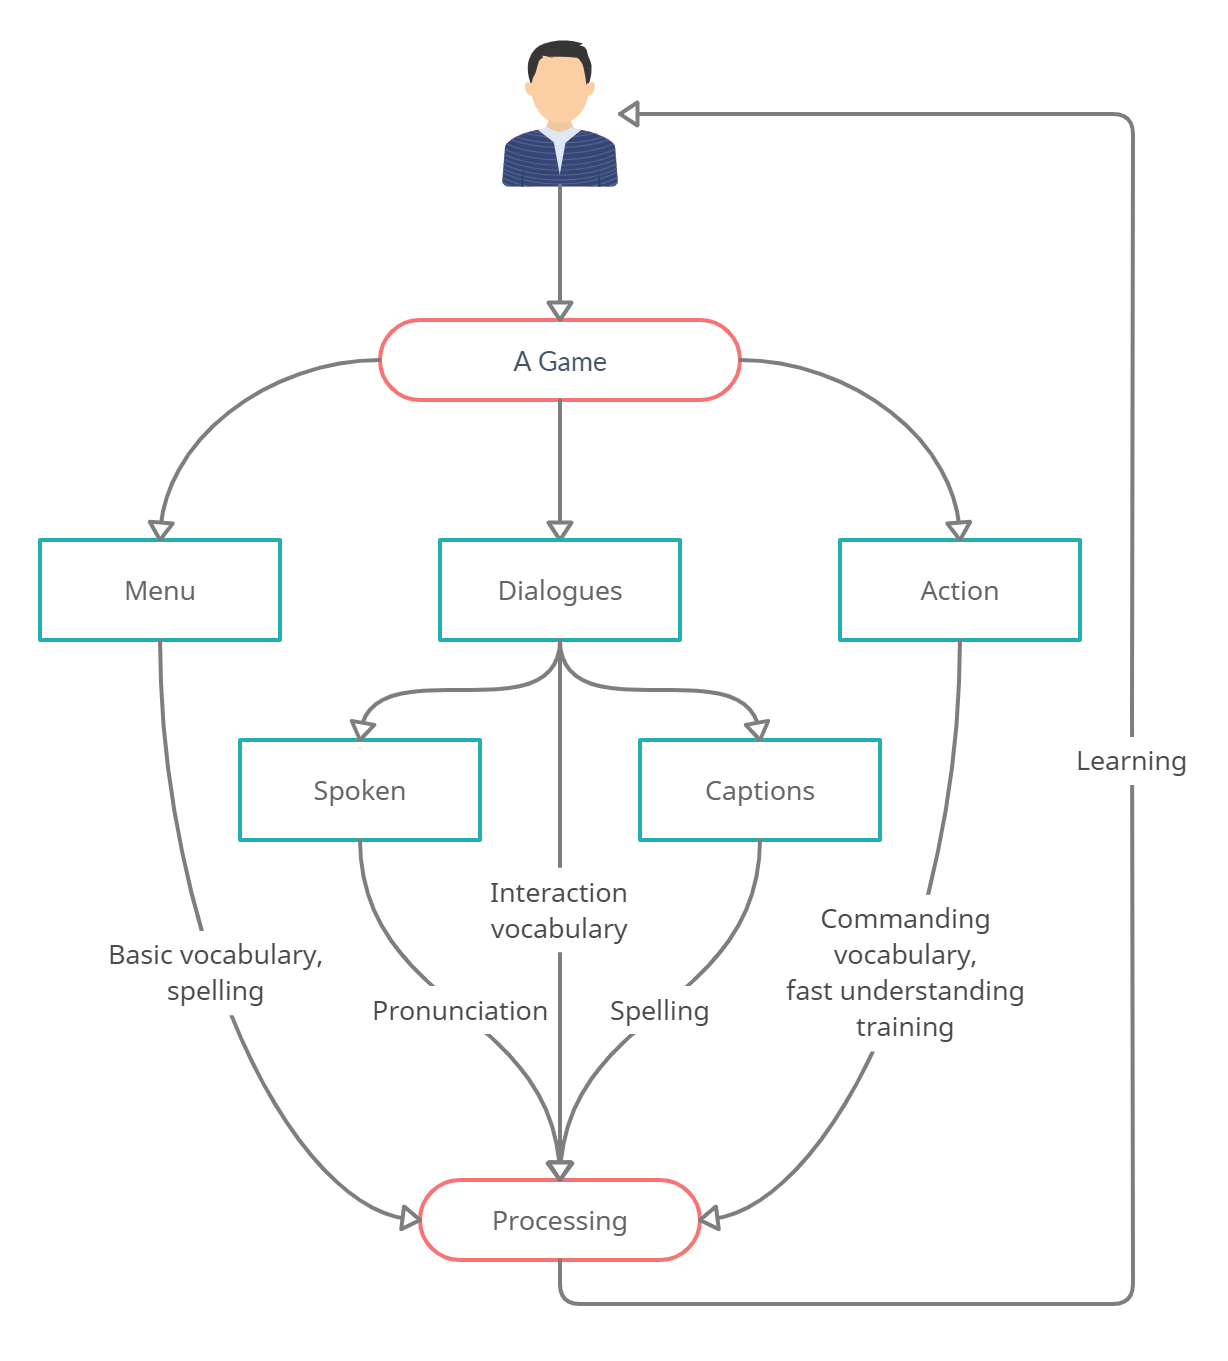
\includegraphics[scale=0.16]{language}
\caption{A diagram of in-game language learning process}
\end{figure}

\section{Negative effects on humans} \label{negative}
People have blamed video games for many bad things since the initial one was made, from bad sight to social anxiety and suicides. While many of these are only biases or prejudices, others of them are, of course, actual facts.

Numerous studies have been done on video game effects during the past 37 years. The reason for this is a growing concern for people's mental and social health. The dangers that people face from playing video games must be emphasized. Even a new video game-related condition called "gaming disorder"~\cite{children,disorder} has been named by the World Health Organization. It is motivated by worries about the risks associated with playing violent games and gaming addiction~\cite{children}.

\subsection{Gaming Disorder and Electronic Nicotine Delivery Systems Dependency} \label{GD and ENDS}
According to a study from 2020, approximately 2 billion individuals worldwide engage in video game play. The worse part is that roughly 1-10\% of the population plays excessively. To properly categorize the harm that video games inflict, the term "gaming disorder" was developed. It was shown that gaming disorder (GD) and other addictive illnesses have many similar characteristics, such as cravings, compulsions, and an unwillingness to stop despite adverse effects~\cite{disorder}.

As mentioned in table 1 (see table 1), the most significant percentage of players are teenagers and young adults. A study shows that an average adolescent plays roughly 1.5 hours daily~\cite{disorder}. It is also necessary to look at the differences between males and females.

Only 35\% of female gamers regularly participate in playing video games, compared to over 75\% of men. Men also often play for more prolonged periods of time, spend more money, and play more frequently than women~\cite{disorder}. 

Excessive video gaming is linked to financial hardship, social and professional issues, and the onset worsening of various mental diseases. In addition to sleep deprivation, day-night reversal, dehydration, malnutrition, obesity, seizures, pressure sores, and a sedentary lifestyle are also affected by these consequences. Excessive video gaming among college students is linked to poorer GPAs, reduced enrollment rates, and trouble sustaining social bonds~\cite{disorder}.

The shocking aspect is that utilizing addictive drugs like alcohol, cigarettes, or ENDS, aka e-cigarettes, is also tightly correlated with playing video games. Although original cigarette smoking among teenagers is generally declining, rates of ENDS usage have risen significantly in recent years. Even though ENDS are considered safer alternatives, they are still dangerous to people's health~\cite{disorder}.

It is also necessary to understand the association between GD and ENDS. Impulsivity, inattention, and sensation-seeking are three indicators of attention-deficit hyperactivity disorder that might be the factors in the relationship between the two dependencies. Due to their lack of inhibition and need for novelty, people with ADHD may be more open to the addictive and highly rewarding stimuli present in video games. Similarly to this, impulsivity's poor self-regulation and self-control may make it harder to allocate the right amount of time and resources to video games. In those with increased impulsivity and ADHD, delay discounting the propensity to choose bigger, later rewards over smaller, more immediate rewards—is frequently disturbed, making them more susceptible to the reinforcement schedules seen in video games and leading to the development of GD~\cite{disorder}.

People with ADHD are more likely to use nicotine, start smoking earlier, and are twice as likely to get addicted to nicotine. Since the stimulant qualities of nicotine mimic those of prescription stimulants allowed to treat ADHD, nicotine in cigarettes and ENDS may be used as self-medication. After starting to smoke, stopping the habit is especially difficult for those who are more impulsive and inattentive, maybe because psychological dysfunction has returned or gotten worse. As a result, there is a common risk for those with ADHD to develop GD/IGD and nicotine dependence~\cite{disorder}.

\subsection{Sexuality problems} \label{sexuality}
Despite the fact that sexually explicit video games are not published by video game console companies, they are frequently found in other games. It is a fact that graphics are improving increasingly over time, and partial nudity is transforming into full nudity in video games. These games are accessible to younger and younger youngsters, and we can already see what a dreadful impact it is having on them. Children being more exposed in public is becoming more widespread, and they are engaging in sexual activity much earlier than generations before them.

\subsection{Bad effects on children} \label{children}
Video games are the main reason why children and adolescents sit in their rooms excessively. They can sit behind their computer or console for hours doing nothing but playing. Because of video games, children are naturally far less inclined to exercise and hang out with their friends, which has a terrible effect on their health and in-person social interactions~\cite{problems}.

\section{Conclusion} \label{conclusion}
It is difficult to categorically state whether video games are beneficial or negative. They undoubtedly have both positive and bad aspects. They may be highly helpful in the areas of education, skill development, language acquisition, and many other things. But it's also important to consider the negatives. On the other hand, video games also have the potential to be quite harmful, whether through addiction, concerns with development as a whole, or problems with sexuality. You can have too much of a good thing, as the adage goes. It's crucial for players to monitor their playtime and maintain a healthy balance between activities.


\bibliography{literatura}
\bibliographystyle{acm}

\newpage
\section*{Comments on the lectures} \label{comments}
\paragraph{Creative writing}The lecture on creative writing was the one I found most fascinating. I appreciated the professor's encouragement not to be afraid to make mistakes. The entire lecture was focused on creating something new, which is crucial in today's quick-paced society. Although it was about writing, the concepts are applicable to producing anything. It's crucial to encourage creativity in others, and I believe that those working in the IT industry especially need to be innovative.
\paragraph{Why should I be an Engineer?}The second highly fascinating lecture was given by our dean, who discussed the benefits of completing a graduate degree. I believe it is good to be aware of all the advantages of the field you are studying to enter the workforce. The salary data he provided was not only fascinating but also inspiring. He also discussed the tasks we must complete before receiving our degrees. He was able to effectively encourage me to keep going despite how difficult and frightening it will be, since, the best is still ahead of me, after all of the hard work.
\paragraph{Bibliography and citation in technical text}Lastly, I found the lecture on bibliography and citation to be really helpful. It's not the most exciting subject, yet academic writing requires it. I wasn't quite sure how to paraphrase, quote, or even work with material from other sources before this class. I believe I now understand how to appropriately reference and paraphrase after listening to our professor's extensive explanation of the subject.

\end{document}
